\documentclass{standalone}
\usepackage{mintikz}

\begin{document}
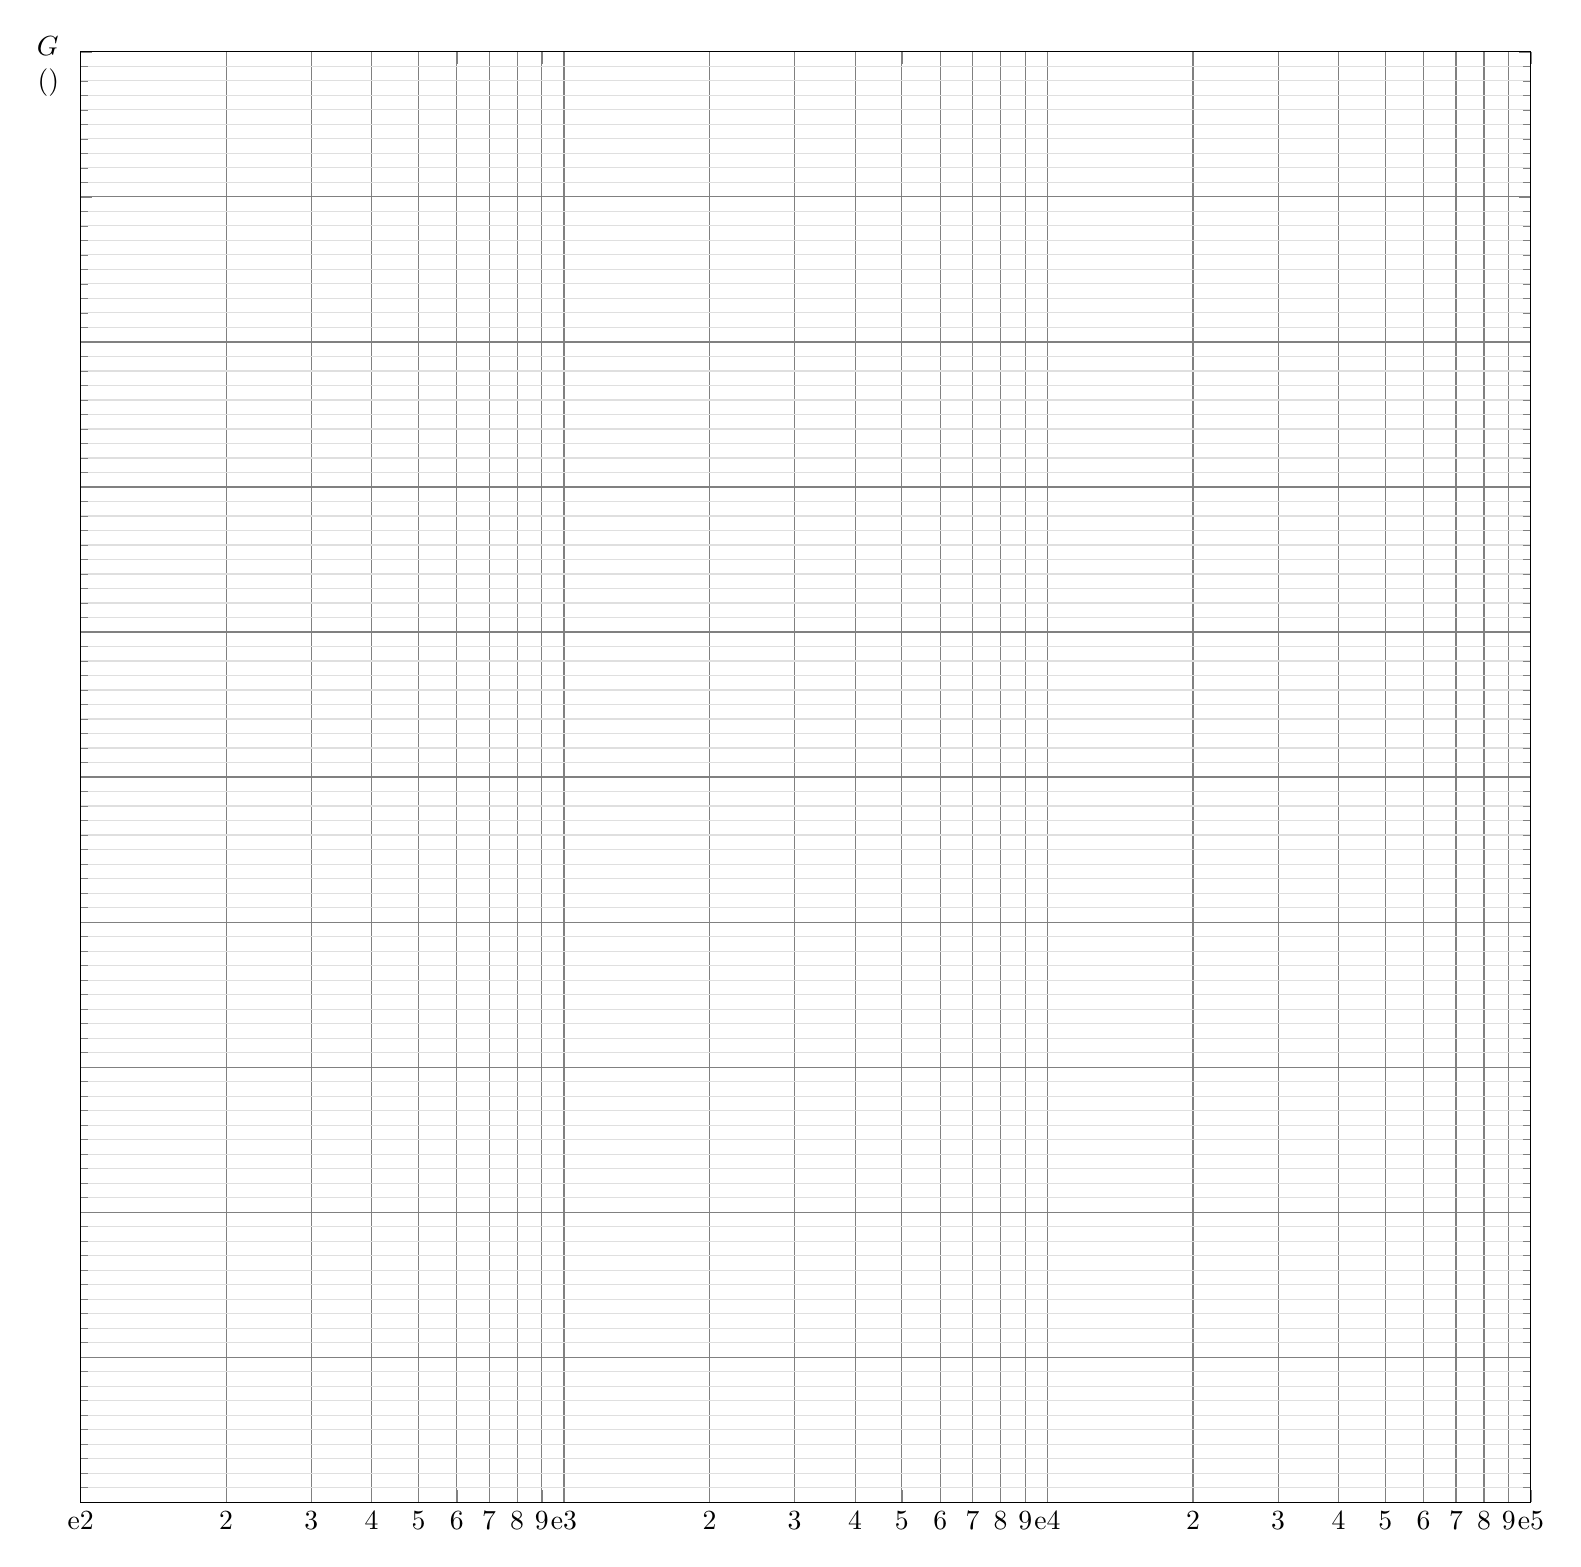
\begin{tikzpicture}
	\begin{semilogxaxis}[
			xmin=1e2, xmax=1e5,
			ymin=0, ymax=100,
			ytick={0, 10, ..., 100},
			yticklabels={},
			minor ytick={1, 2, ..., 99},
			% extra y tick style={yticklabels={}, gray!25},
			log ticks with fixed point,
			xtick={
					1e2, 2e2, 3e2, 4e2, 5e2, 6e2, 7e2, 8e2, 9e2,
					1e3, 2e3, 3e3, 4e3, 5e3, 6e3, 7e3, 8e3, 9e3,
					1e4, 2e4, 3e4, 4e4, 5e4, 6e4, 7e4, 8e4, 9e4,
					1e5},
			xticklabels={
					\num{e2}, 2, 3, 4, 5, 6, 7, 8, 9,
					\num{e3}, 2, 3, 4, 5, 6, 7, 8, 9,
					\num{e4}, 2, 3, 4, 5, 6, 7, 8, 9,
					\num{e5}},
			width=20cm, height=20cm,
			grid=both,
			minor grid style={gray!25},
			major grid style={black!50},
			clip=false
		]
		\node[anchor=east, align=center]
		at (axis cs:95,99) {$G_{\dB}$\\$(\si{\dB})$};
	\end{semilogxaxis}
\end{tikzpicture}
\end{document}
